\documentclass[11pt, oneside]{article}   	% use "amsart" instead of "article" for AMSLaTeX format
\usepackage[margin=1in]{geometry}               % See geometry.pdf to learn the layout options. There are lots.
\geometry{letterpaper}                   	% ... or a4paper or a5paper or ... 
%\geometry{landscape}                		% Activate for rotated page geometry
%\usepackage[parfill]{parskip}    		% Activate to begin paragraphs with an empty line rather than an indent
\usepackage{graphicx}				% Use pdf, png, jpg, or eps§ with pdflatex; use eps in DVI mode
						% TeX will automatically convert eps --> pdf in pdflatex		
\usepackage{amssymb}
\usepackage{amsmath}
\usepackage{array}
\usepackage{indentfirst}
\usepackage{enumitem}
\usepackage{mathptmx}
\usepackage{float}

%SetFonts

%SetFonts

\setcounter{secnumdepth}{3} % default value for 'report' class is "2"

\title{APPM 4560 Laboratory 2 Report}
\author{Rhys Olsen\\
\texttt{rhys.olsen@colorado.edu}
 \and Jessica Petty\\
 \texttt{jessica.petty@colorado.edu}
 }
\date{November 16, 2016}

\begin{document}
\maketitle
\section{Simulating a homogenous Poisson process (HPP)}
\subsection{Representation of $T(1), \dots, T(n)$}
The random variables $T(1), \dots, T(N)$ represent the times of the arrivals of the HPP on the domain $[0, t]$. Note that while $[0, t]$ is pre-determined by the way the problem is posed, $N$ is a random variable based on how many arrivals the simulation generates on $[0, t]$ and is \emph{not} pre-determined.

%At each iteration, a new random variable$\sim \text{Exponential}(\lambda)$ is generated and added to the previous arrival time. In this way, each inter-arrival time has a distribution Exponential$\lambda$), thus satisfying the conditions of an HPP. 
\subsection{Distribution of the Random Number $N$}
As $N$ represents the number of arrivals of a Poisson process in a time window of size $t - 0 = t$, $N \sim \text{Poisson}(\lambda t)$.
\subsection{Representation of the Quantity $T(N+1)$}
As $T(N)$ is defined as the time of the last arrival of the HPP in time interval $[0, t]$, $T(N + 1)$ represents the time of the first arrival of the HPP \emph{after} time $t$.
\subsection{Distribution of the Quantity $T(N+1)-t$}
The random variable $T(N + 1) - t$ is the amount of time taken after $t$, the end of the interval, until the next arrival of the HPP. Each individual arrival of the HPP, including $T(N + 1)$, is exponentially distributed with rate paramater $\lambda$ by assumption. Since $T(N)$ is the time of the \emph{last} arrival of the HPP on $[0, t]$, we have that $T(N + 1) > t$. By the memoryless property, $P(T(N + 1) > t + s | T(N + 1) > t) = P(T(N + 1) > s)$, which amounts to saying that $T(N + 1) - t \sim \text{Exp}(\lambda)$
\subsection{Comparing the Distributions of $T(N+1)-T(N)$ and $T(N+1)-t$}
The random variables $T(N + 1) - t$ and $T(N + 1) - T(N)$ do \emph{not} have the same distribution.

Observe that $T(N)$ is the maximum among $U_1, \dots, U_N \sim_{\text{i.i.d.}} \text{Uniform}(0, t)$, so:
$$P(T(N) < t) = P(U_1 < t, \dots, U_N < t)$$
which by independence is:
$$P(U_1 < t) \times \dots \times P(U_N < t)$$
and as $P(U_1 < t), \dots,  P(U_N < t)$ are all identically distributed, for $U \sim \text{Uniform}(0, t)$, this is simply:
$$P(U < t)^n = \left( \int_{0}^{t} p_U(x) \mathrm{d}x \right)^n = \left(\frac{t}{t}\right)^n = 1^n = 1$$

Thus we always have that $T(N) < t \Rightarrow T(N + 1) - T(N) > T(N + 1) - t$. In other words, knowledge about the time interval $[0,t]$ affects the expected distribution of arrivals within that interval.
\subsection{Developing the Probability Density Function of $T(N+1)$}
Having argued that $T(N + 1) - t \sim \text{Exp}(\lambda)$, we expect $T(N + 1) \sim \text{Exp}(\lambda) + t$. To justify this, we derive the probability density function $f_{T(N + 1)}(x)$.

As $T(N)$ is by definition the last arrival time of the process before or during time $t$, it is not possible for $T(N + 1)$ to occur before or during time $t$. Thus $f_{T(N + 1)}(x) = 0$ for $x \leq t$. By the memoryless property of the exponential distribution, $P(T(N + 1) = t + s | T(N + 1) > t) = P(T(N + 1) = s)$, where the condition $T(N + 1) > t$ is given by the problem defintion. Moreover, on the a posteriori assumption that any further time increment $r$ elapses before $T(N + 1)$, the memoryless property also shows that $P(T(N + 1) = t + r + s | T(N + 1) > t + r) = P(T(N + 1) = s)$. The only distribution that could satisfy these properties is an exponential with rate parameter $\lambda$ known to be greater than $t$, which is simply an exponential with rate paramater $\lambda$ shifted $t$ increments to the right. Thus:
\[
f_{T(N + 1)}(x) =
\begin{cases} 
      0 & x \leq t \\
      \lambda e^{-\lambda (x - t)} & x > t 
   \end{cases}
\]
\subsection{Simulation of a Homogenous Poisson Process with Rate Parameter $\lambda=3$}
\subsubsection{Analysis of Simulation of $N$}
The values generated for $N$ after 10K simulations are consistent with our results in part (1.2). We said that $N \sim \text{Poisson}(\lambda t)$ for $\lambda=3$, $t = 4$. We see this consistency in two ways. Over an interval $[0,t]$, the number of arrivals of the HPP $N(t) \sim \text{Poisson}(\lambda t)$ and the expected value of a Poisson with rate $\lambda$ is $\lambda$. Therefore, over the interval $[0,4]$ with $\lambda=3$, the expected number of arrivals is 12, which is consistent with our simulations. Furthermore, the plot below displays the 10K simulations alongside the theoretical Poisson distribution. Clearly, the plot confirms the distribution of $N$ as being Poisson($\lambda t$). 
\begin{figure}[H]
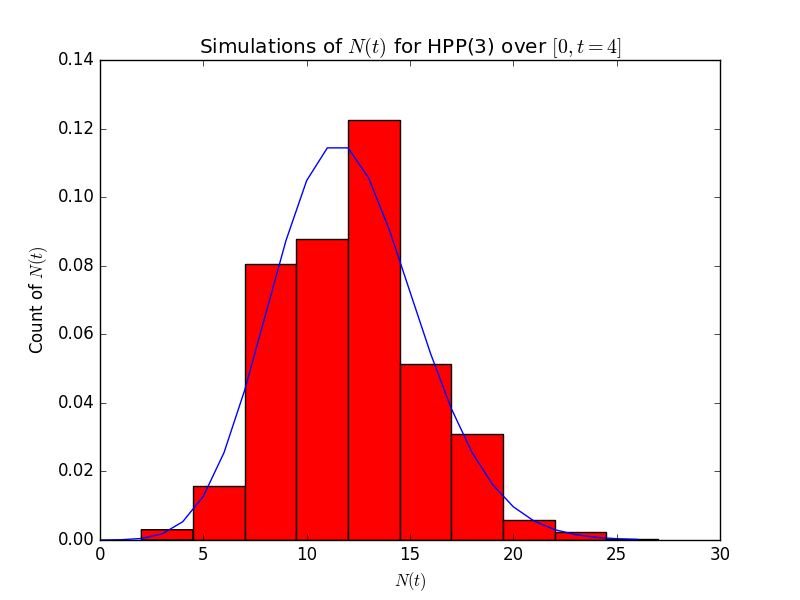
\includegraphics[scale=.5]{hpp_nt}
\caption{The results of 10,000 simulations of $N$, the number of arrivals over $[0,4]$ for the HPP with intensity $\lambda=3$ beside the probability mass function of a random variable $\sim \text{Poisson}(\lambda t)$ with $\lambda=3$ and $t=4$.}
\label{fig:x}
\end{figure}

\subsubsection{Simulation of $T(N+1)-T(N)$ and $T(N+1)-t$ and Corresponding Analysis}
Once again, the results of 10K simulations of $T(N+1)-T(N)$ and $T(N+1)-t$ are consistent with the ideas presented in part (1.5). We detailed that $T(N+1)-T(N)$ and $T(N+1)-t$ did not have the same distribution, which is clear from their corresponding plots. The results of 10K simulations of $T(N+1)-T(N)$ is plotted beside an Exponential random variable with rate $\lambda=3$. As can be observed, the bins of the histogram do \emph{not} match the expected distribution of the exponential variable. Compare that to the results of 10K simulations of $T(N+1)-t$. These results are expected to take a distribution Exponential($\lambda$) where $\lambda=3$. This time, the theoretical distribution matches closely to the observed phenomenon. This confirms the claim that $T(N+1)-T(N)$ and $T(N+1)-t$ do not have the same distribution.
\begin{figure}[H]
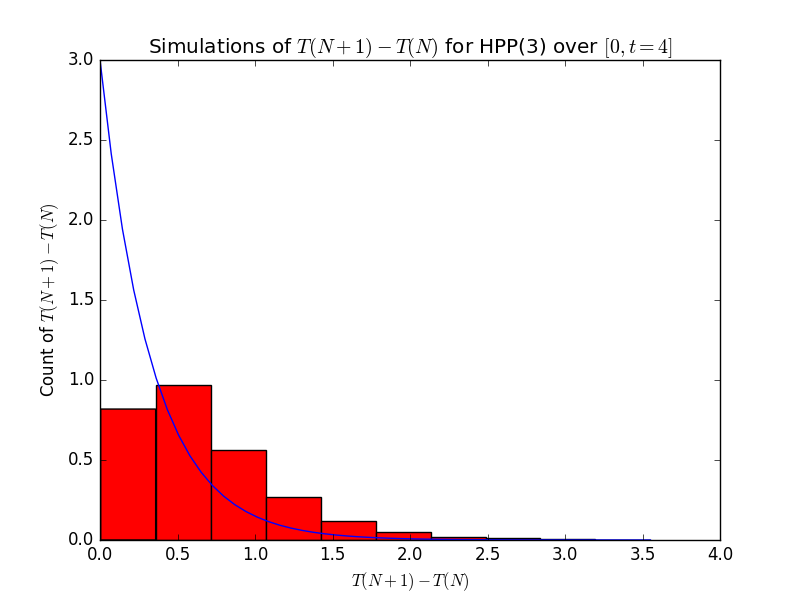
\includegraphics[scale=.45]{hpp_tn1_tn}
\caption{The results of 10,000 simulations of $T(N+1)-T(N)$, the inter-arrival time between the last arrival on the interval $[0,4]$ and the first arrival after the interval. The displayed plot of the theoretical distribution of an Exponential with $\lambda=3$ does not match the results of the simulation.}
\label{fig:x}
\end{figure}

\begin{figure}[H]
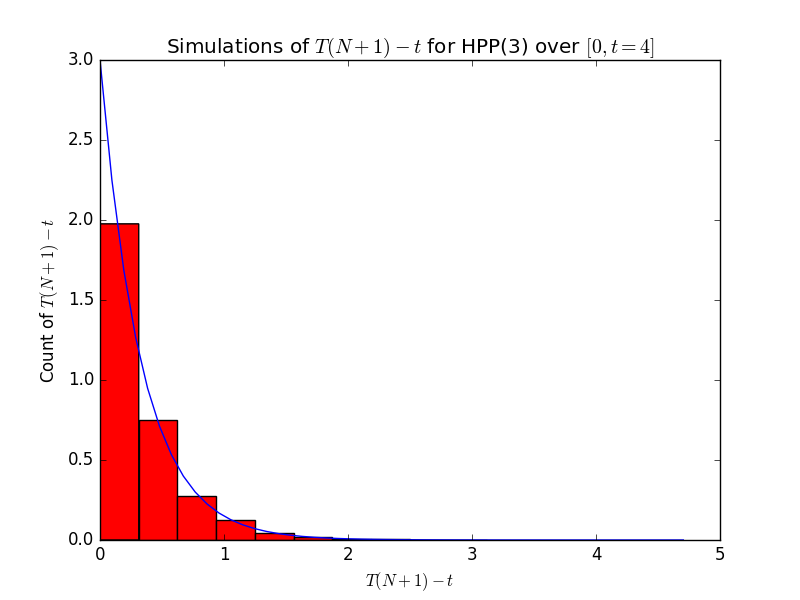
\includegraphics[scale=.45]{hpp_tn1_t}
\caption{The results of 10,000 simulations of $T(N+1)-t$, the time between the first arrival after the end of the interval $[0,t]$ and t, beside the expected theoretical distribution, an Exponential with $\lambda=3$.}
\label{fig:x}
\end{figure}

\subsubsection{Simulation and Analysis of $T(N+1)$}
The claim in part (1.6) was that the probability density function $f_{T(N+1)}(x)$ for $T(N+1)$ was 0 for times $x \leq t$ and $\lambda e^{-\lambda (x - t)}$ otherwise. Clearly, the plot of this theoretical expectation is consistent with the results of the simulation. Observe that the simulated counts of $T(N+1)$ is in fact 0 for all times less than $t$, then closely matches the expected probability density function $f_{T(N+1)}(x)$.
\begin{figure}[H]
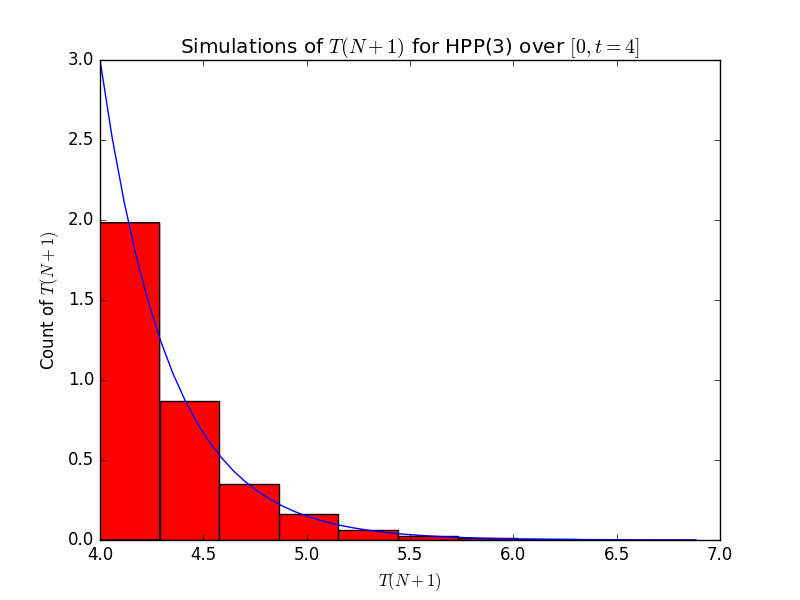
\includegraphics[scale=.5]{hpp_tn1}
\caption{The results of 10,000 simulations of $T(N+1)$, the time of the first arrival of the HPP after the interval $[0,4]$, beside the expected probability density function $f_{T(N+1)}(x)=\lambda e^{-\lambda (x - t)}$.}
\label{fig:x}
\end{figure}

\section{Simulating a Non-homogenous Poisson Process (NHPP)}
\subsection{Algorithm to Simulate a Non-homogenous Poisson Process}
The algorithm to simulate a non-homogenous Poisson process with intensity function $\lambda(t)$ over an interval $[0,T]$ is as follows:
\begin{enumerate}[leftmargin=30pt,labelindent=65pt,itemindent=30pt]
\item[\textsc{step 1:}] Calculate the maximum $C$ of the function $\lambda(t)$ on the interval $[0,T]$
\item[\textsc{step 2:}] Set $i:=0$, $T(0):=0$, and $N:=0$
\item[\textsc{step 3:}] Generate $U_1 \sim \text{Uniform}(0,1)$
\item[\textsc{step 4:}] Set $i:=i+1$ and $T(i) := T(i-1) - \ln(U_1)/C$
\item[\textsc{step 5:}] Generate $U_2 \sim\text{Uniform}(0,1)$
\item[\textsc{step 6:}] If $T(i) > t$, set $N:=N-1$ and stop. Otherwise, if $U_2 \leq \frac{\lambda(T(i))}{C}$, set $N:=N+1$. Go to Step 3.
\end{enumerate}

\subsection{Theoretical Distribution of $W$ and Expected Value of $W$}
$W$ represents the random number of arrivals in the time interval $[0, T]$ of a non-homogenous Poisson process with rate function $\lambda(t)$. The mean function corresponding to this rate function is $\Lambda(t) = \int_{0}^{t}\lambda(s)\mathrm{d}s $. Now, the expected number of arrivals $W$ of a non-homogenous Poisson process with intensity function $\lambda(t)$ over the interval $[0, T]$ has a theoretical distribution Poisson($\Lambda(T)$).

Given a non-homogenous Poisson process with intensity function $\lambda(t)=t^2-10t+26$, the corresponding mean function is $\Lambda(t)=\int_{0}^{t}\lambda(s)\mathrm{d}s=\left[\frac{s^3}{3} - 5s^2 + 26s + C\right]_{0}^{t} =\frac{t^3}{3}-5t^2+26t$. Over the interval $[0,9]$, the mean function evaluates to $\Lambda(9)=\frac{9^3}{3} - 5(9)^2+26(9) = 72$. Therefore, the random variable $W$ has a theoretical distribution $\text{Poisson}(72)$.

Additionally, the expected value of a Poisson distribution with rate parameter $\lambda$ is simply $\lambda$. Therefore, for the random variable $W \sim \text{Poisson}(72)$, $\mathbb{E}[W]=72$.

\subsection{Simulation and Analysis of Arrivals of a Non-homogenous Poisson Process}
After 10K simulations of a non-homogenous Poisson process with rate function $\lambda(t) =t^2-10t+26$ over the interval $[0,9]$, the simulated number of arrivals, $W$ in that interval is plotted and analyzed. The histogram displaying the observed counts of $W$ is compared with the probability mass function of a Poisson distribution with rate $\lambda = 72$. This p.m.f. represents the theoretical distribution of $W$, and as can be seen from the plot, the theoretical distribution matches the results of the simulations very closely. Furthermore, if $W \sim \text{Poisson}(72)$, one would expect to observe an average of 72 arrivals over the interval. The simulated average value for $W$ is 71.6909, further supporting our analysis of the distribution of $W$.
\begin{figure}[H]
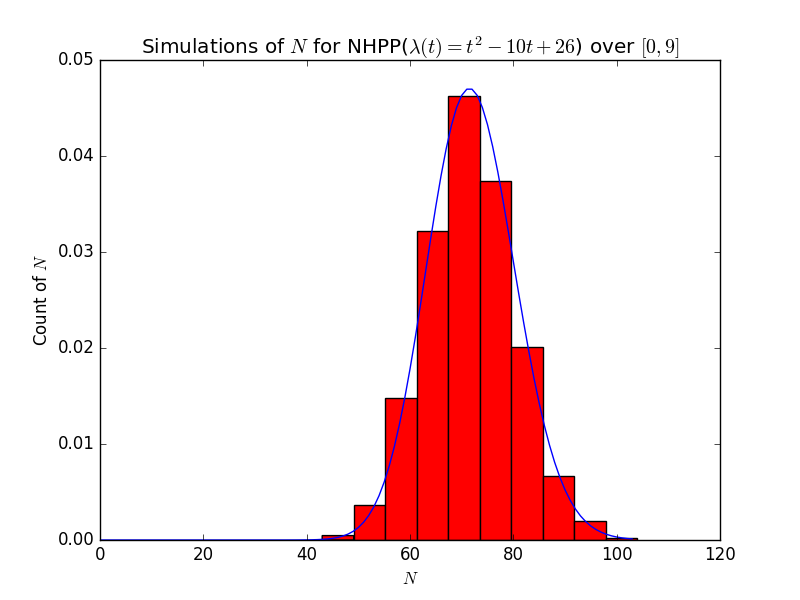
\includegraphics[scale=.5]{nhpp_n}
\caption{The results of 10,000 simulations of $W$, the number of arrivals on $[0,9]$ for a non-homogenous Poisson process with rate function $\lambda(t)=t^2-10t+26$. These results are plotted beside the probability mass function of a Poisson random variable with rate $\lambda=72$, the expected distribution of $W$.}
\label{fig:x}
\end{figure}

\end{document}
